\documentclass[brazil]{beamer}
\usepackage{beamerthemesplit}
\usepackage[brazilian]{babel}
\usepackage[utf8]{inputenc}
\usepackage{color}
\usepackage{xcolor}
\usepackage{graphicx}
%\usepackage{subcaption}
\usepackage{float}
\usepackage{wrapfig}
\usepackage{amssymb}
\usepackage{amsmath}
\usepackage{fancybox}
\usepackage{ulem}
\usepackage{listings}
\usepackage{upquote}
\setbeamertemplate{footline}[frame number]
\usetheme{Dresden}

%http://tex.stackexchange.com/questions/100838/beamer-dresden-theme-miniframes-appeareance-and-frame-number-insertion
\newcommand{\frameofframes}{/}
\newcommand{\setframeofframes}[1]{\renewcommand{\frameofframes}{#1}}
\setframeofframes{of}
\makeatletter
\setbeamertemplate{footline}
  {%
    \begin{beamercolorbox}[colsep=1.5pt]{upper separation line foot}
    \end{beamercolorbox}
    \begin{beamercolorbox}[ht=2.5ex,dp=1.125ex,%
      leftskip=.3cm,rightskip=.3cm plus1fil]{author in head/foot}%
      \leavevmode{\usebeamerfont{author in head/foot}\insertshortauthor}%
      \hfill%
      {\usebeamerfont{institute in head/foot}\usebeamercolor[fg]{institute in head/foot}\insertshortinstitute}%
    \end{beamercolorbox}%
    \begin{beamercolorbox}[ht=2.5ex,dp=1.125ex,%
      leftskip=.3cm,rightskip=.3cm plus1fil]{title in head/foot}%
      {\usebeamerfont{title in head/foot}\insertshorttitle}%
      \hfill%
      {\usebeamerfont{frame number}\usebeamercolor[fg]{frame number}\insertframenumber~\frameofframes~\inserttotalframenumber}
    \end{beamercolorbox}%
    \begin{beamercolorbox}[colsep=1.5pt]{lower separation line foot}
    \end{beamercolorbox}
  }
\makeatother

\usefonttheme{structurebold}

\begin{document}

  \title{Metaballs no PBRT}
  \author{Vinícius Vendramini e Wilson Kazuo Mizutani}

  \frame{
    \titlepage
  }
  
  \section{Introdução}
  
    \subsection{}
    
      \begin{frame}
        \frametitle{Revisando definição}
        \begin{itemize}
          \pause
          \item
            Dado um threshold $T$ e $N$ elementos com
            \begin{itemize}
              \item Posição $P_i \in \mathbb{R}^3$
              \item Raio $R_i > 0$
              \item Fator de aglomeração $B_i < 0$
            \end{itemize}
          \pause
          \item A contribuição de cada elemento é dado por
                \vspace{.5em}
                \begin{center}
                  $D_i(x) = Te^{\frac{B}{R^2}*r_i(x)^2 - B}$ \\
                  onde \\
                  $r_i(x) = \| x - P_i \| $
                \end{center}
                \vspace{.5em}
          \pause
          \item A função implícita de uma metaball fica
                \vspace{.5em}
                \begin{center}
                  $F(x) = \sum\limits_{i} D_i(x) - T$
                \end{center}
        \end{itemize}
      \end{frame}
      
      % Efeito dos parâmetros
      
      \begin{frame}
        \frametitle{Duas possibilidades}
        \begin{enumerate}
          \item
            Calcular intersecção do raio com o objeto
            \begin{itemize}
              \item Mais fiel à definição
              \item Não tem solução explícita
              \item Restrições no PBRT
            \end{itemize}
          \vspace{1em}
          \pause
          \item Gerar um mesh
            \begin{itemize}
              \item Método dos \textit{marching cubes}
              \item Depende da granularidade dos voxels usados
            \end{itemize}
        \end{enumerate}
      \end{frame}
      
  \section{Calculando intersecção}
  
    \subsection{}
    
      \begin{frame}
        \frametitle{Algoritmo proposto por Blinn}
          Converge para a intersecção usando uma margem de erro
          \begin{itemize}
            \vspace{1em}
            \pause
            \item
              Método híbrido
              \begin{itemize}
                \item Iteração de Newton
                \item \textit{Regula falsi}
              \end{itemize}
            \vspace{1em}
            \pause
            \item
              Itera até que $| D(ray(t)) - T | < \varepsilon $, para algum $\varepsilon$ determinado
            \vspace{1em}
            \pause
            \item Adaptado para considerar raios que ``saem'' do objeto também
          \end{itemize}
      \end{frame}
      
      \begin{frame}
        \frametitle{Dificuldades}
        Não há uma forma paramétrica geral para metaballs
        \begin{itemize}
          \vspace{1em}
          \pause
          \item
            Restrições do PBRT
            \begin{itemize}
              \item Intersecção com raio deve fornecer
                    $\frac{\partial p}{\partial u}$,
                    $\frac{\partial p}{\partial v}$,
                    $\frac{\partial n}{\partial u}$ e
                    $\frac{\partial n}{\partial v}$
              \item Também precisa implementar os métodos
                    \textbf{Area()}, \textbf{Pdf()} e \textbf{Sample()}
            \end{itemize}
          \vspace{1em}
          \pause
          \item
            Como contornar?
            \begin{itemize}
              \item Tangentes: sabemos como fornecer o valor em si, mas não
                    haveria $u$ e $v$ associados (sempre zero, por exemplo)
              \item Area, pdf e amostragem: ?
            \end{itemize}
        \end{itemize}
      \end{frame}
      
      %Permite calcular as normais
  
  \section{Gerando uma mesh}
  
    \subsection{}
    
      \begin{frame}
        \frametitle{Algoritmo dos \textit{marching cubes}}
        Divide o espaço em um cubo de voxels
        \begin{itemize}
          \vspace{1em}
          \item
            Em cada posição do cubo, verifica quais vértices $v$ satisfazem
            \vspace{1em}
            \begin{center}
              $F(v) > 0$
            \end{center}
          \pause
          \vspace{1em}
          \item
            256 casos
            \begin{itemize}
              \item Usa uma máscara de 8 bits para indexar uma tabela
              \item Pode ser reduzido a 15 casos
            \end{itemize}
          \vspace{1em}
          \pause
          \item Gera uma malha de triângulos que aproxima o objeto
        \end{itemize}
      \end{frame}
    
      \begin{frame}
        \frametitle{Resultado parcial}
        \begin{center}
          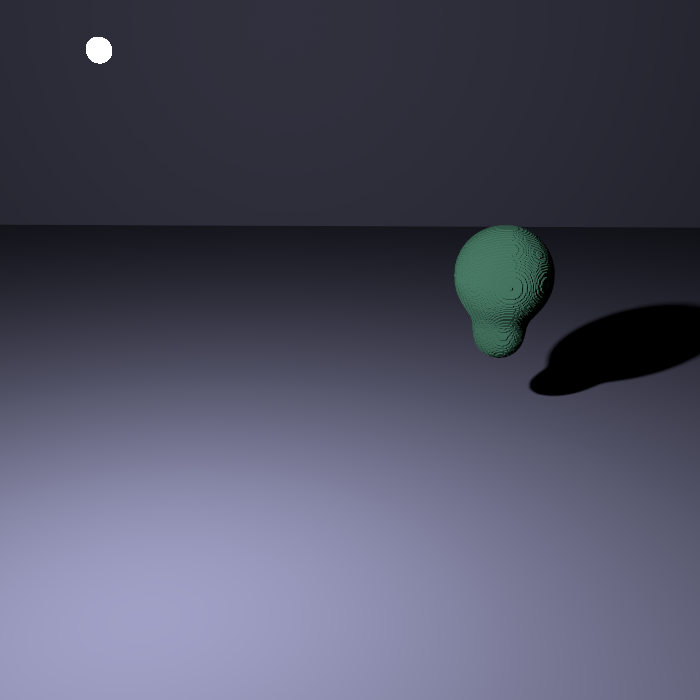
\includegraphics[width=.6\textwidth]{imgs/metaball-preview.png}
        \end{center}
      \end{frame}
  
\end{document}
